\begin{figure*}[ht]
    \begin{center}
        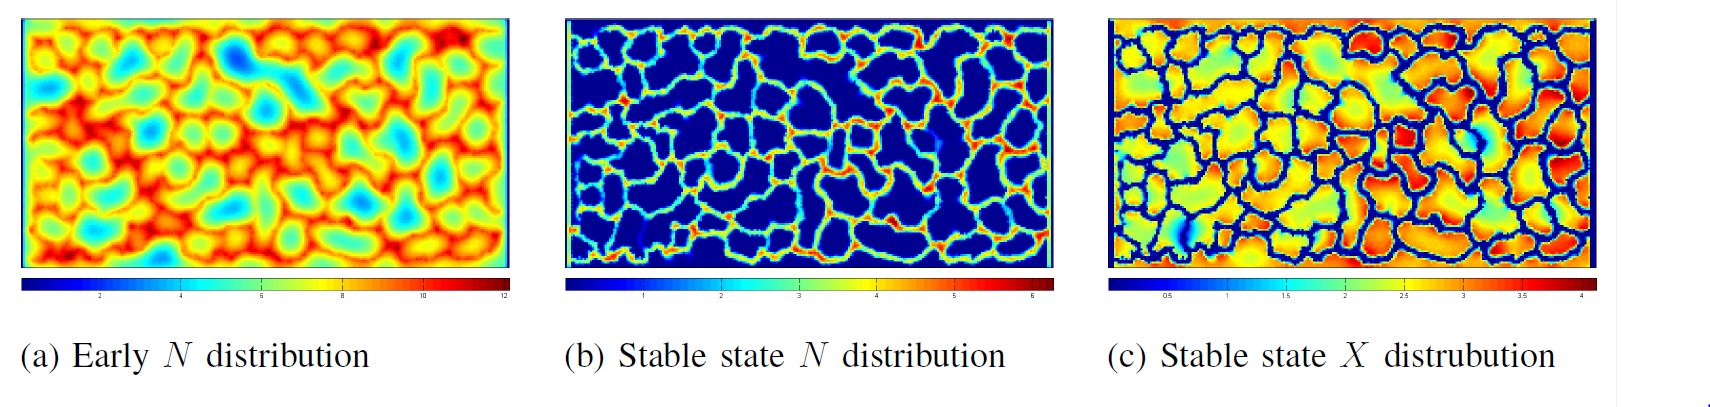
\includegraphics[width=\textwidth]{./figures/Figure7.JPG}
    \end{center}
    \caption{\textbf{Cell culture activation}: The distribution of nutrient (a) when
    the vessel flow begins, but the supported cells are not yet active, (b) at steady
    state nutrient distribution when the supported cells are active; note that all
    extra-vessel nutrient is consumed, (c) the product distribution when the
    supported cells are active.}
    \vspace{+1mm}
    \label{runningFactory}
\end{figure*}

The quality of the network is evaluated by determining the flow through each branch
and modeling the release of nutrients and the capture of secretions from the
supported cells. A full description of the functioning vascular model and its
derivation is given in \cite{Davis2017Exploiting}. To assess the health of the
supported cells given a running vascular network, the rate of metabolism of each
supported cell is estimated by measuring how efficiently the cells produce some
arbitrary product, $X$, described by Equation~\ref{productProduction}.

\begin{equation}
    \frac{\partial X}{\partial t}=+\mu _{p}  \frac{N}{(N+k_p)} \frac{k_i}{(X+k_i)}
    M_p + D_{p}\bigtriangledown^{2} X
    \label{productProduction}
\end{equation}

Where $M_p$ is supported cell biomass. To produce a realistic model of cellular
metabolism, the parameter values of the supported cells is replicated from
\cite{delindavis:Bernard1999Mass} and is based on vanillin production of Pycnoporus
cinnabarinus. The product $X$ is secreted by the supported cells consuming nutrient
$N$ following Michaelis-Menten kinetics with a reaction rate of $\mu _{p}$, where the
saturation of enzymes involved in the $X$ production is considered $k_p$. The
negative feedback due to product inhibition is also taken into account, with a
correspondent inhibitor constant $k_i$ \cite{Han1988Extended},
\cite{Levenspiel1980Monod} and \cite{Aiba1968Kinetics}.

%\input{modelTable}

Nutrient will be consumed by the supported cells in direct correspondence to the
production of $X$, but at a different reaction rate $\mu_n$:

\begin{equation}
    \frac{\partial N}{\partial t}=-\mu _{n}  \frac{N}{(N+k_p)} \frac{k_i}{(k_i+X)}
    M_p + D_{p}\bigtriangledown^{2} N
    \label{nutrientConsumption}
\end{equation}

Figure~\ref{runningFactory} illustrates the distribution of nutrient and product
during simulated network operation for the network illustrated in
Figure~\ref{phaseOne}(c).
Figure~\ref{runningFactory}(a) illustrates the nutrient distribution before the
supported cells have become active. In Figure~\ref{runningFactory}(b) gives the
nutrient distribution following supported cell activation. In
Figure~\ref{runningFactory}(c) the distribution of the product is illustrated. Note
the regions of low product (the blue areas) where the vascular flow is limited.

The final step is to integrate the amount of $X$ extracted from the cellular culture
by the vascular network over a fixed period, in this case two hours. This
accumulation of product will be a function of the aggregate metabolic rate of the
supported cells. It is this value the simulator returns as the fitness score of the vascular network architecture.




